\subsection{Kiến trúc Hệ thống}
\label{subsec:system_architecture_impl}

Kiến trúc tổng thể của hệ thống VieVu khi triển khai là sự kết hợp giữa ứng dụng client (Flutter), nền tảng Backend as a Service (Supabase) và một backend tùy chỉnh (Python/FastAPI) cho các tác vụ chuyên biệt. Sơ đồ Hình~\ref{fig:system_architecture} minh họa các thành phần chính và luồng tương tác dữ liệu giữa chúng.

\begin{figure}[H]
    \centering
    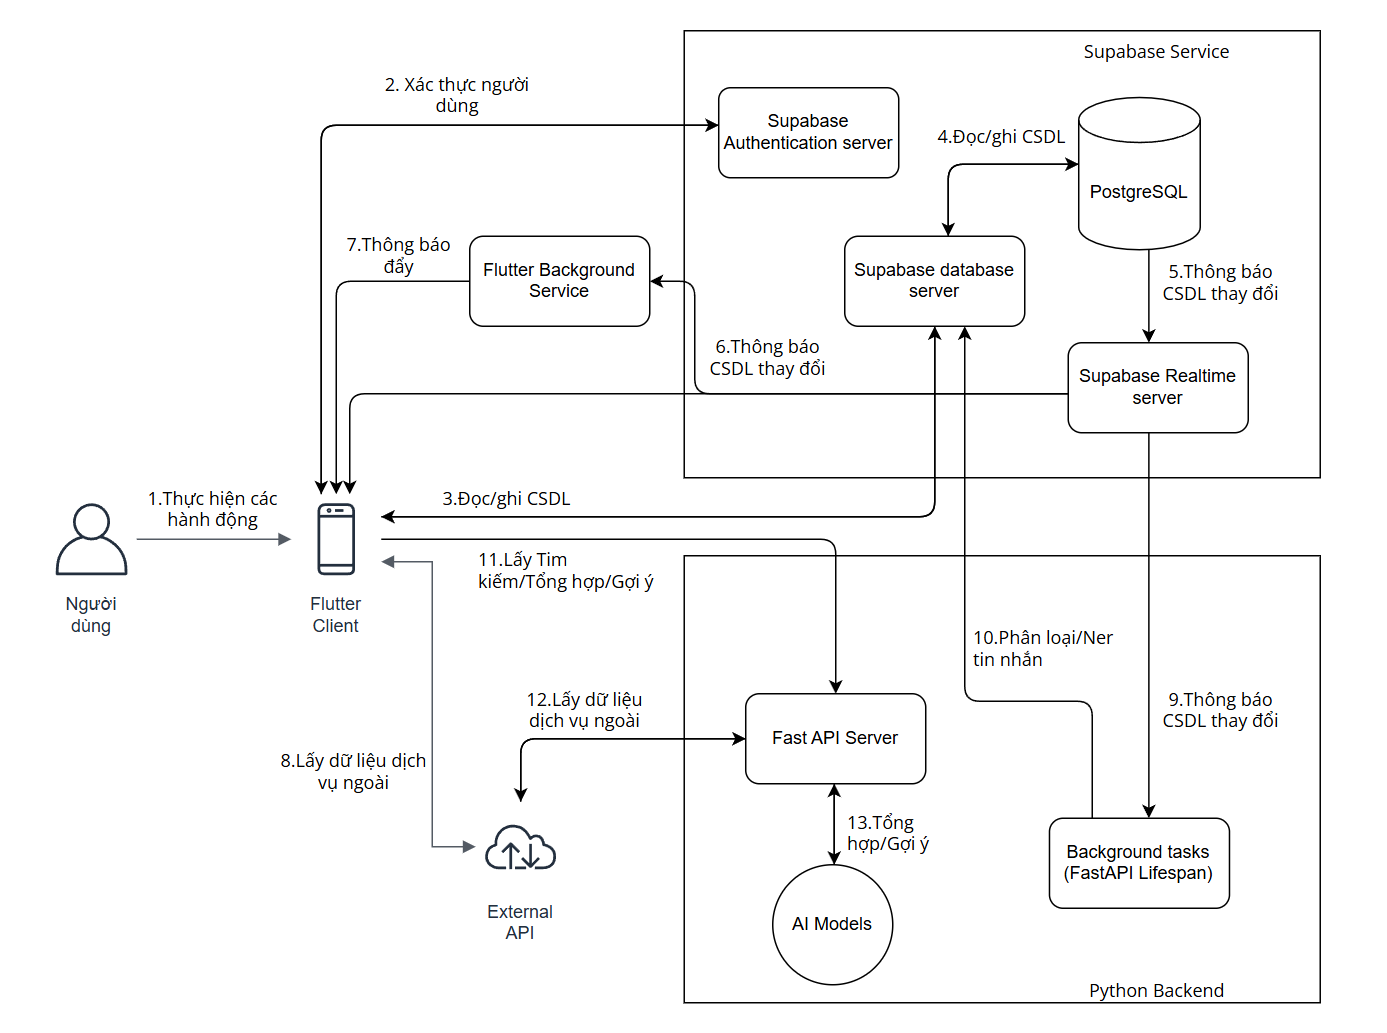
\includegraphics[width=1\textwidth]{figures/c4/architecture.png}
    \caption{Kiến trúc tổng thể của hệ thống VieVu.}
    \label{fig:system_architecture}
\end{figure}
\begin{enumerate}
    \item \textbf{Người dùng (User):} Tác nhân chính tương tác với hệ thống thông qua ứng dụng client.
    \item \textbf{Flutter Client:} Ứng dụng di động được xây dựng bằng Flutter, là giao diện chính để người dùng thực hiện các hành động như xem thông tin, lập kế hoạch, nhắn tin, yêu cầu gợi ý, v.v.
    \item \textbf{Flutter Background Service:} Một dịch vụ chạy nền trên thiết bị người dùng (triển khai bằng Flutter), có thể dùng để xử lý thông báo hoặc đồng bộ dữ liệu nền tảng.
    \item \textbf{Supabase Service:} Nền tảng BaaS cung cấp các dịch vụ backend cốt lõi, bao gồm:
        \begin{itemize}
            \item \texttt{Supabase Authentication server:} Xử lý xác thực người dùng.
            \item \texttt{Supabase database server:} Cung cấp API để tương tác trực tiếp với CSDL PostgreSQL.
            \item \texttt{PostgreSQL Database:} Nơi lưu trữ dữ liệu chính của ứng dụng.
            \item \texttt{Supabase Realtime server:} Quản lý các kết nối thời gian thực và phát các thay đổi dữ liệu.
        \end{itemize}
    \item \textbf{Python Backend:} Backend tùy chỉnh được xây dựng để xử lý các tác vụ phức tạp, bao gồm:
        \begin{itemize}
            \item \texttt{FastAPI Server:} Cung cấp các API endpoint cho các chức năng AI và tìm kiếm/tổng hợp.
            \item \texttt{AI Models:} Các mô hình AI/ML đã huấn luyện (NN gợi ý, NER, ZSC,v.v.) được tải và sử dụng bởi FastAPI server.
            \item \texttt{Background tasks (FastAPI Lifespan):} Tác vụ nền chạy bất đồng bộ bao gồm phân loại, nhận dạng tên, để tiền xử lý tin nhắn.
        \end{itemize}
    \item \textbf{External API:} Các API của bên thứ ba (ví dụ: Trip.com, Ticketbox) mà Python Backend tương tác để lấy dữ liệu.
\end{enumerate}




\noindent Kiến trúc kết hợp này cho phép VieVu tận dụng các dịch vụ mạnh mẽ, sẵn có và khả năng mở rộng của Supabase cho các tác vụ phổ thông, đồng thời sử dụng một backend Python/FastAPI tùy chỉnh, linh hoạt để triển khai các thuật toán AI/ML phức tạp và tích hợp với các nguồn dữ liệu bên ngoài, tạo nên một hệ thống hoàn chỉnh và hiệu quả.